% Soubory musí být v kódování, které je nastaveno v příkazu \usepackage[...]{inputenc}

\documentclass[
  12pt,
	t,
	aspectratio=1610,
	unicode,
]{beamer}

\usepackage[utf8]{inputenc}
\usepackage{graphicx}
\usepackage[nohyperlinks]{acronym}
\usepackage{cmap}
\usepackage{booktabs}
\usepackage{amsmath}

\input{nastaveni}
\date{červen 2026}

\pdfsettings
\hypersetup{pdfpagemode=FullScreen}

\usetheme{VUT}
\logoheader

\begin{document}

\setbeamertemplate{navigation symbols}{}
\begin{frame}[plain,c]
	\begin{center}
		\vspace{1em}
		{\Large Vysoké učení technické v Brně}\\[0.4em]
		{\large Fakulta elektrotechniky a komunikačních technologií}\\[2.2em]
		{\huge Návrh měřiče impedance}\\[1.2em]
		{\large Bakalářská práce}\\[2.0em]
		\begin{tabular}{rl}
			Autor: & Vojtěch Glombíček\\
			Vedoucí: & Ing. Alexandr Otáhal, Ph.D.\\
		\end{tabular}\\[2.0em]
		Brno, červen 2026
	\end{center}
\end{frame}

\begin{frame}
	\frametitle{O čem práce je}
	\begin{columns}[T]
		\begin{column}{0.54\textwidth}
			\textbf{Cíl:} navrhnout a ověřit digitální měřič impedance pro pasivní součástky.
			\vspace{0.5em}
			\begin{itemize}
				\item Frekvenční rozsah $100\,\mathrm{Hz}$ až $100\,\mathrm{kHz}$
				\item Měření $R$, $L$, $C$ z amplitudy a fáze
				\item Komunikace s PC přes USB/sériovou linku
			\end{itemize}
			\vspace{0.5em}
			\textbf{Výstup práce:} funkční prototyp, firmware, PC aplikace a ověřovací měření proti LCR metru BK Precision 880.\par
		\end{column}
		\begin{column}{0.46\textwidth}
			\centering
			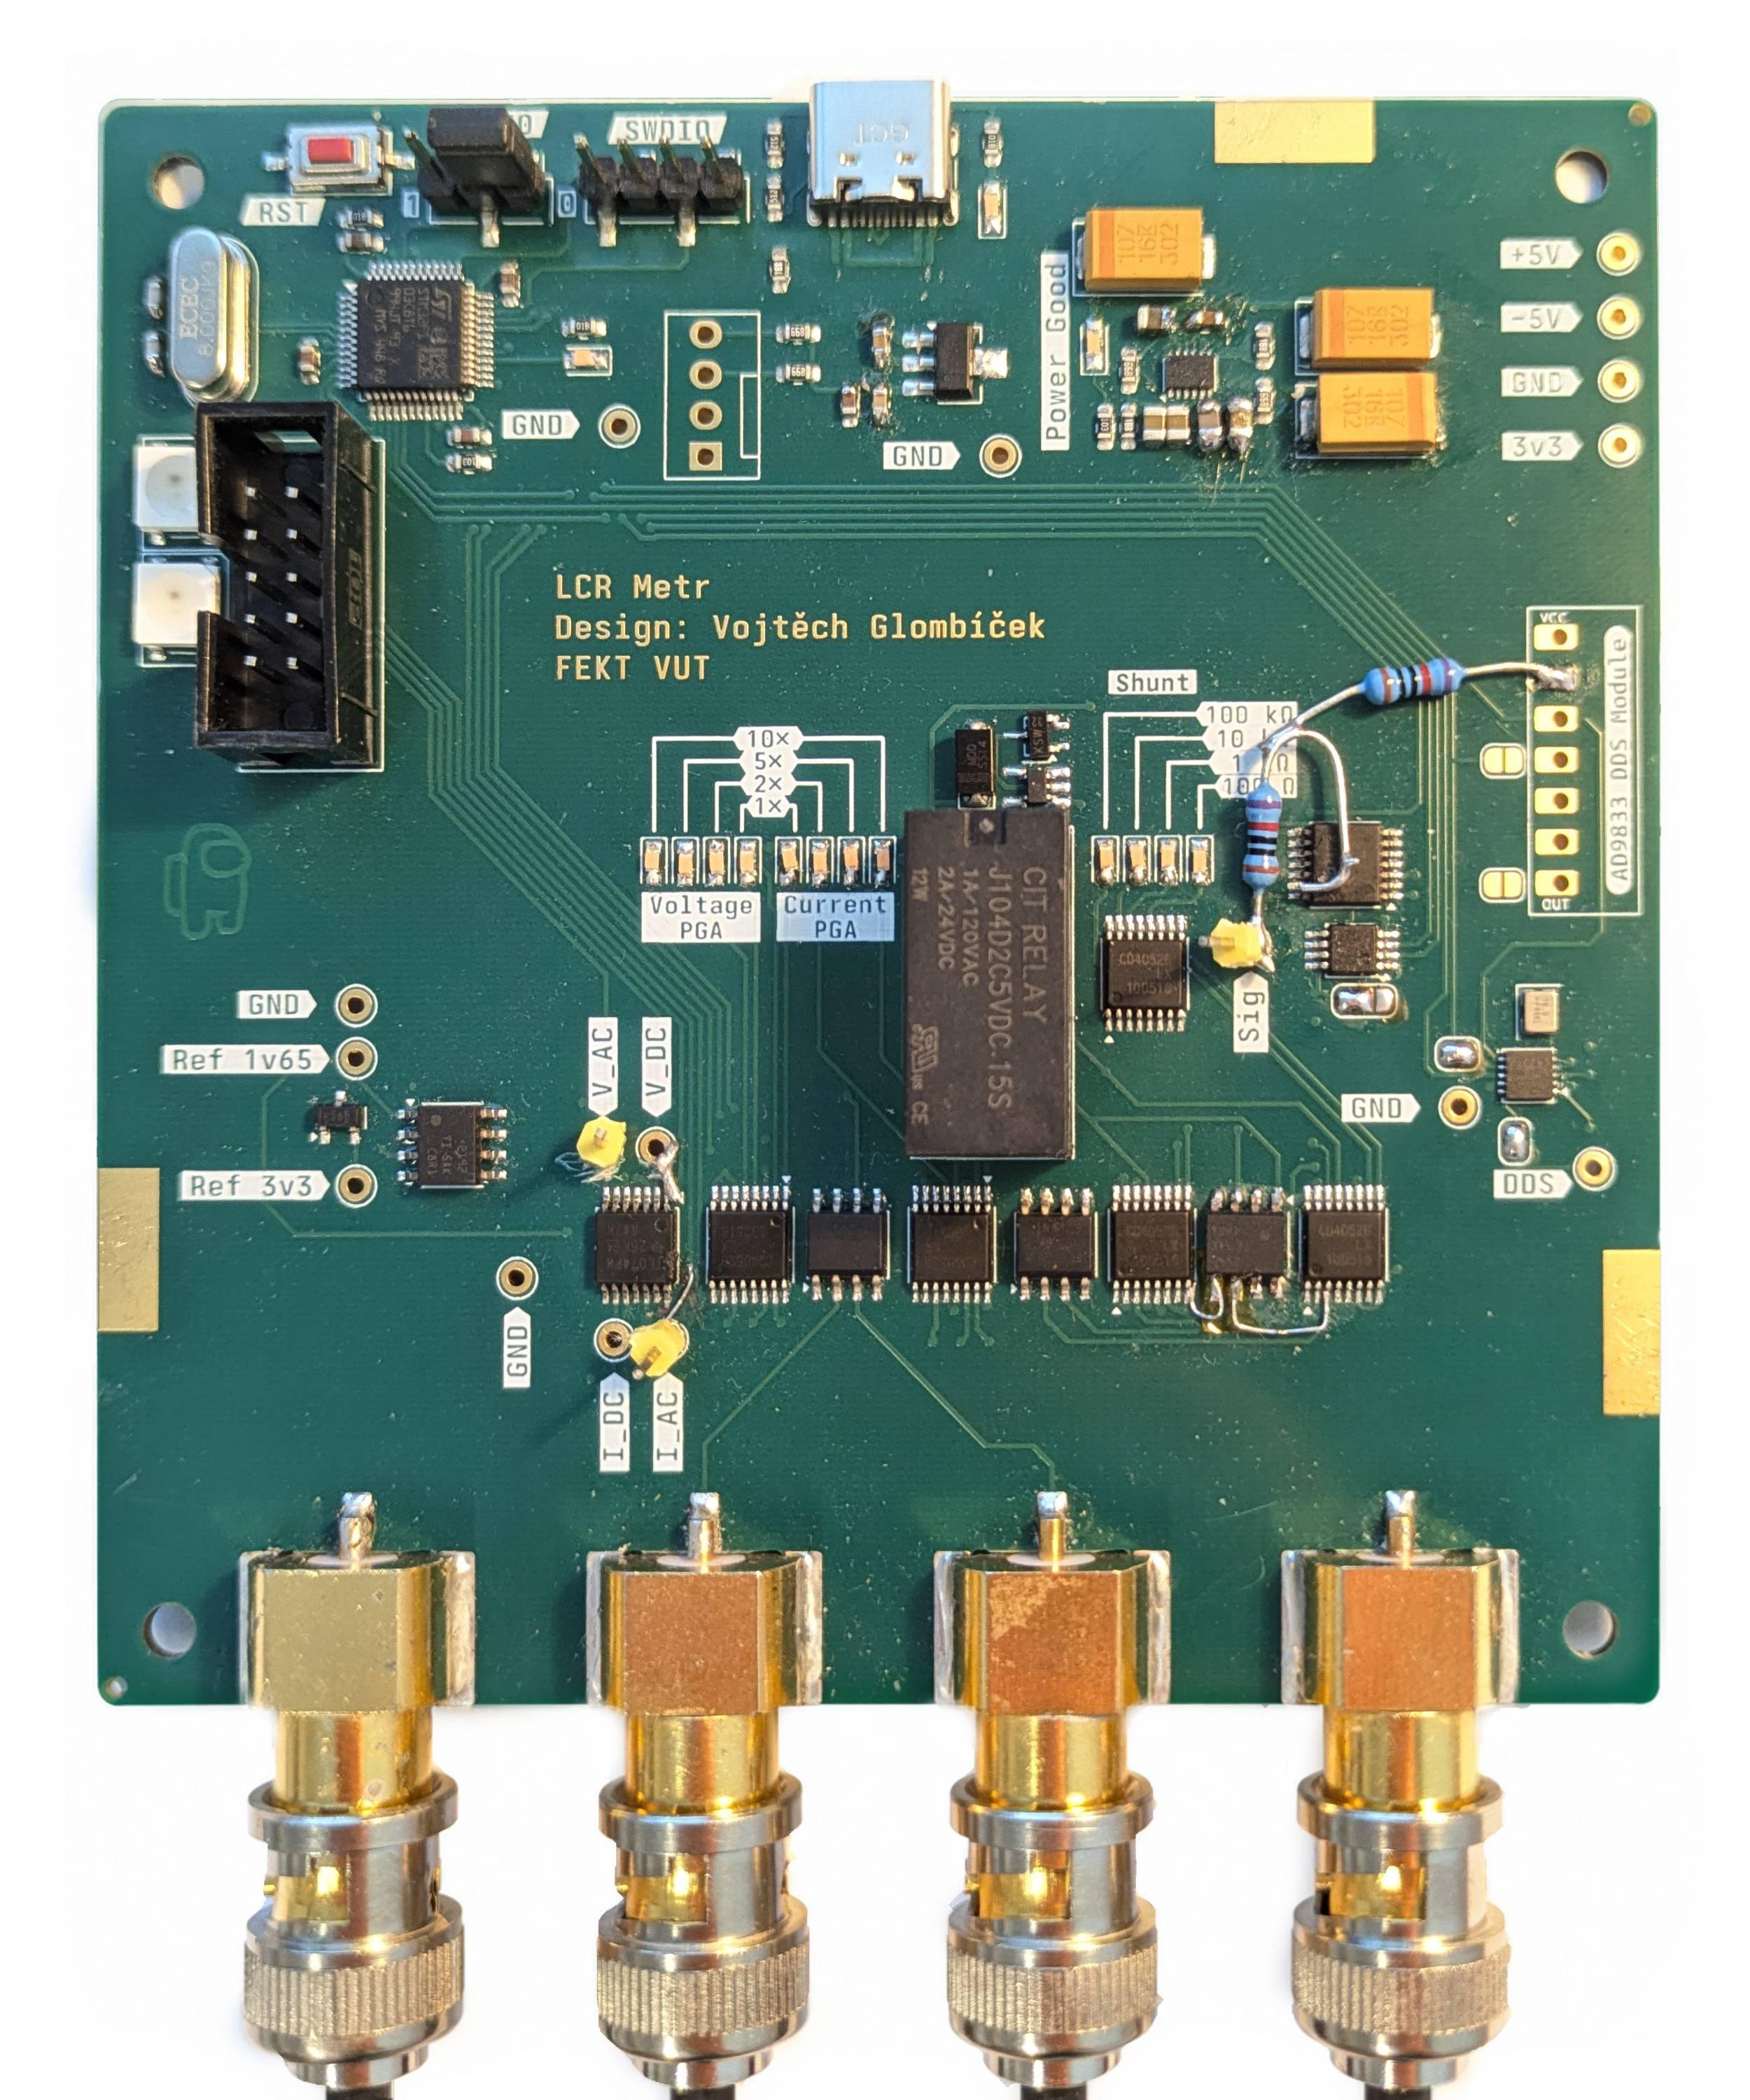
\includegraphics[width=0.72\columnwidth,height=0.58\textheight,keepaspectratio]{obrazky/final_PCB_photo.jpg}\par
		\end{column}
	\end{columns}
\par
\end{frame}

\begin{frame}
	\frametitle{Základní princip měření}
	\small
	\begin{columns}[T]
		\begin{column}{0.50\textwidth}
			\textbf{Zvolená metoda: samovyvažovací můstek}
			\begin{itemize}
				\item Měřená součástka je buzena sinusovým signálem
				\item Proud se převádí na napětí přes známý bočník
				\item Z poměru amplitud a fázového posunu se vypočte komplexní impedance
			\end{itemize}
			\vspace{0.8em}
				\[
					|Z| = \frac{U_x}{U_r} R_r,\qquad
					Z = |Z|\angle\varphi
				\]
			\end{column}
				\begin{column}{0.50\textwidth}
					\centering
					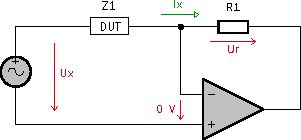
\includegraphics[width=0.86\columnwidth,height=0.28\textheight,keepaspectratio]{obrazky/i_v_conv.pdf}
					\vspace{0.25em}
					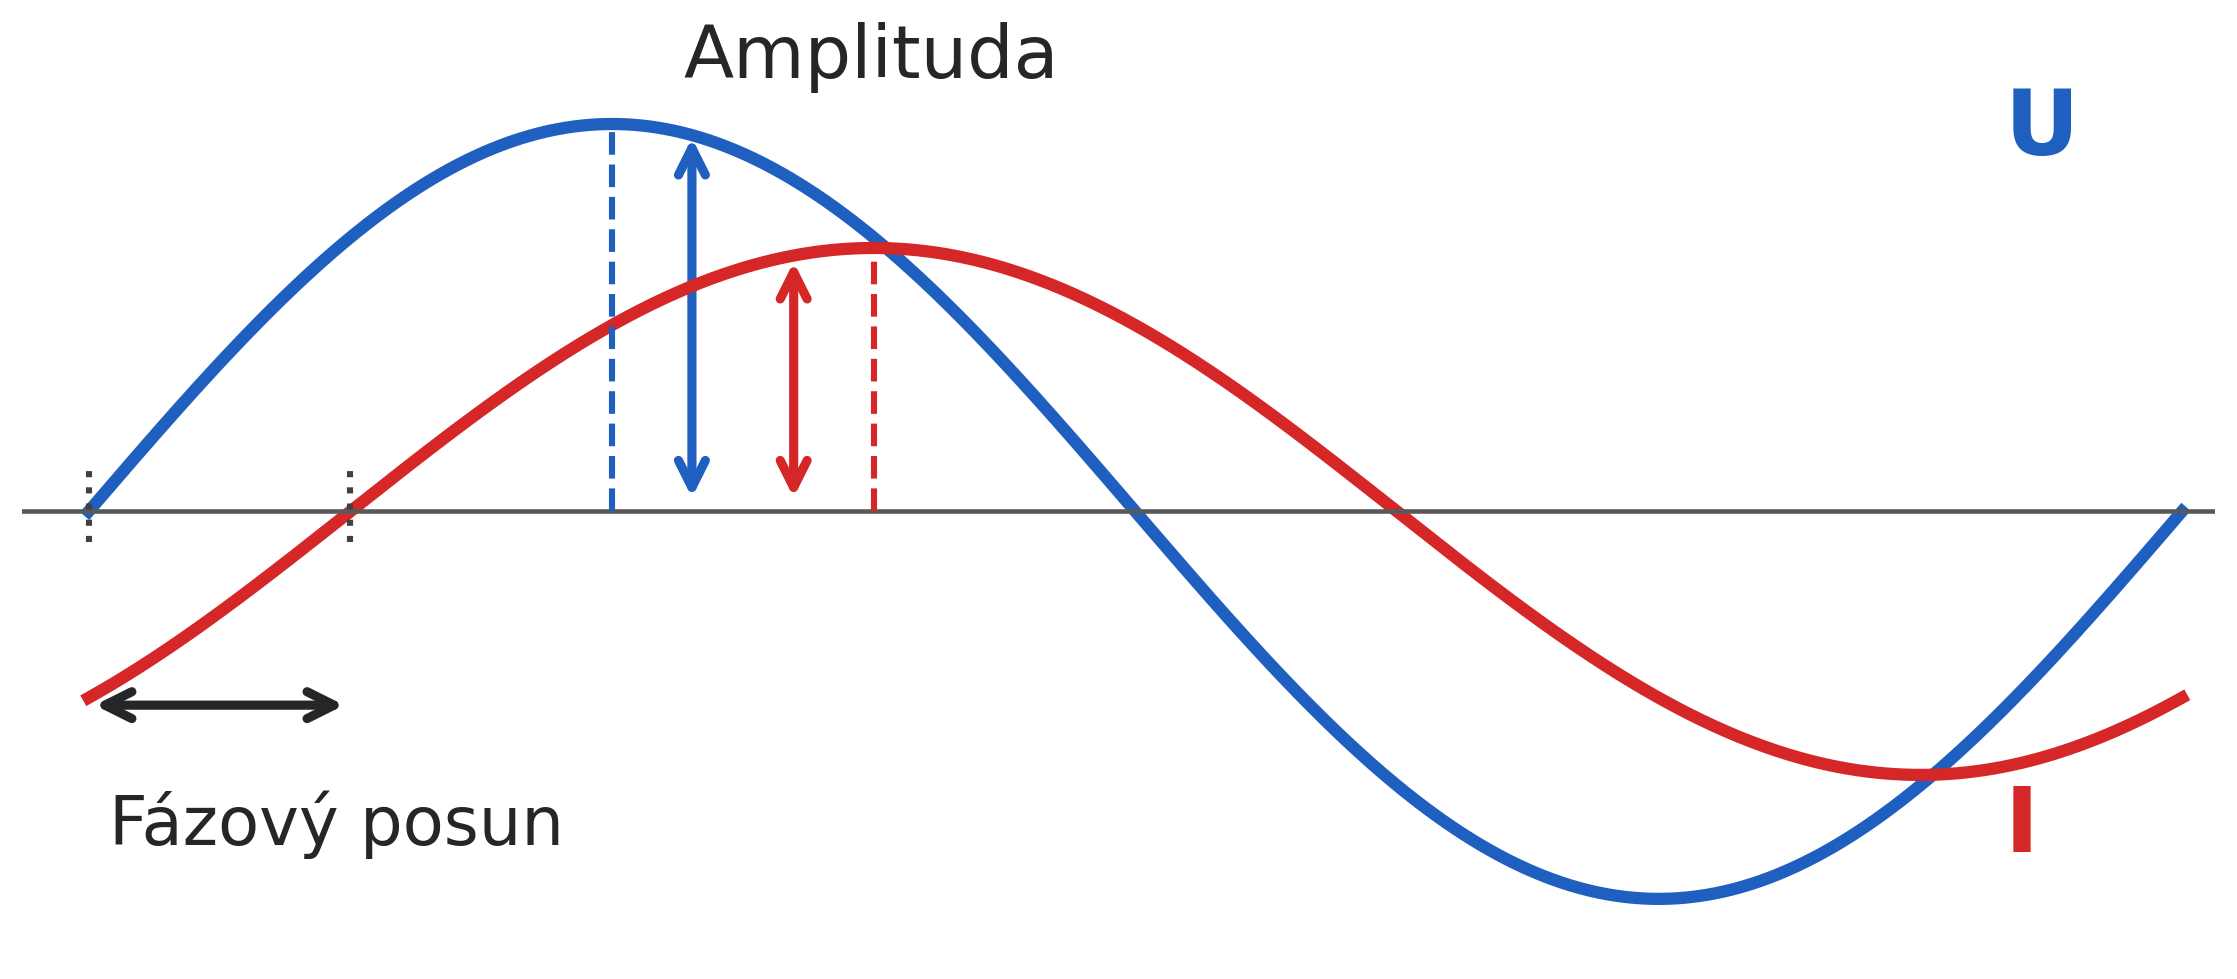
\includegraphics[width=\columnwidth,height=0.30\textheight,keepaspectratio]{obrazky/voltage_current_phase.png}
			\end{column}
	\end{columns}
\end{frame}

\begin{frame}
	\frametitle{Architektura navrženého přístroje}
	\small
	\begin{columns}[T]
		\begin{column}{0.42\textwidth}
			\begin{enumerate}
				\item DDS generátor vytvoří měřicí sinus
				\item Analogová část upraví amplitudu a offset
				\item Měřicí můstek převede proud na napětí
				\item Dva ADC kanály vzorkují napětí a proud
				\item MCU vypočte amplitudy, fázi a impedanci
			\end{enumerate}
		\end{column}
		\begin{column}{0.58\textwidth}
			\centering
				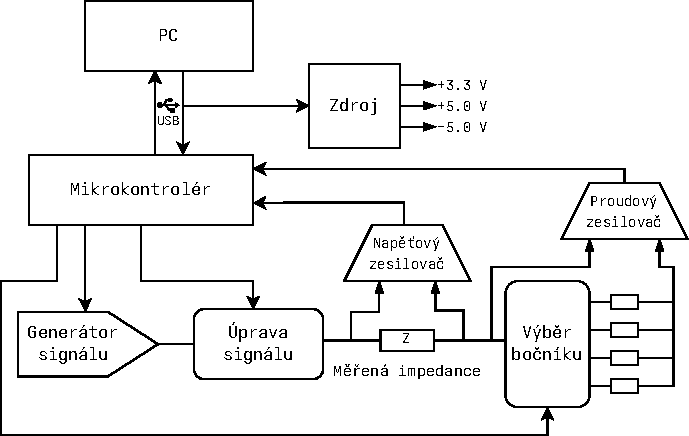
\includegraphics[width=\columnwidth,height=0.58\textheight,keepaspectratio]{obrazky/block_diagram_meter.pdf}
		\end{column}
	\end{columns}
\end{frame}

\begin{frame}
	\frametitle{První prototyp a poučení}
	\begin{columns}[T]
		\begin{column}{0.48\textwidth}
			\textbf{Ověřovaný koncept}
			\begin{itemize}
				\item Analogové vyhodnocení amplitudy a fáze
				\item Špičkový detektor pro amplitudu
				\item XOR detektor pro fázový posun
				\item Jednoduché zpracování pomocí ADC
			\end{itemize}
				\vspace{0.3em}
				\begin{alertblock}{Problém}
					Testování ukázalo citlivost na šum, zkreslení signálu a nedostatečně spolehlivé měření fáze.
				\end{alertblock}
				\textbf{Důsledek:} přechod na přímé vzorkování harmonických signálů.
			\end{column}
			\begin{column}{0.52\textwidth}
				\centering
				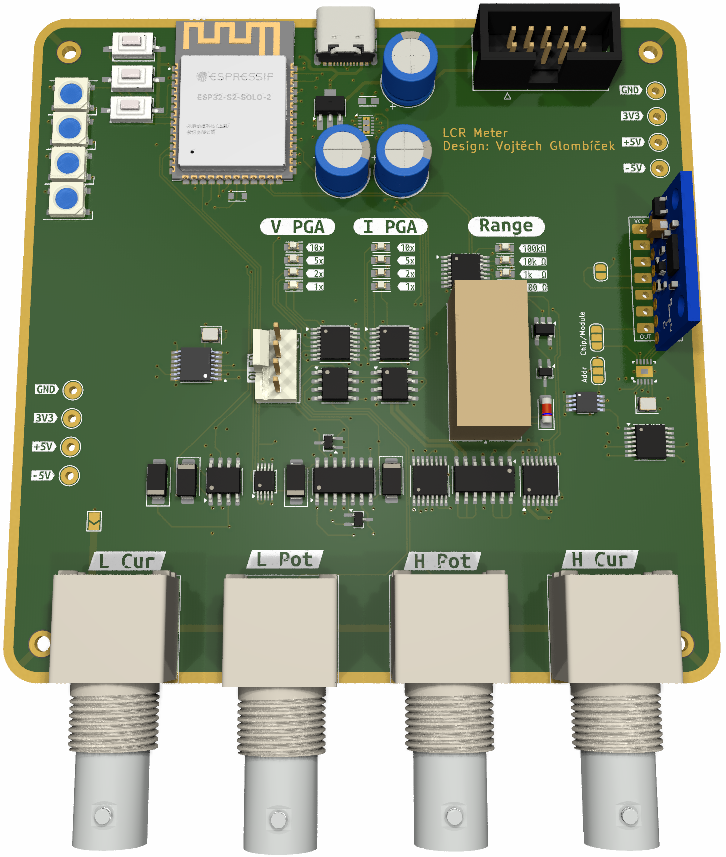
\includegraphics[width=\columnwidth,height=0.64\textheight,keepaspectratio]{obrazky/prototyp_render.png}
		\end{column}
	\end{columns}
\end{frame}

\begin{frame}
	\frametitle{Přímé vzorkování a výpočet}
	\begin{columns}[T]
		\begin{column}{0.43\textwidth}
			\begin{itemize}
				\item Napěťový i proudový signál se přímo vzorkují ADC
				\item Z naměřených dat se pomocí DFT vytáhne pouze složka na nastavené měřicí frekvenci
				\item Z této složky se určí amplituda a fáze obou kanálů
				\item Rušení mimo měřicí frekvenci má menší vliv na výsledek
			\end{itemize}
			\vspace{0.2em}
			\textbf{Výhoda:} selektivní vyhodnocení bez analogového fázového detektoru.
		\end{column}
		\begin{column}{0.57\textwidth}
			\centering
			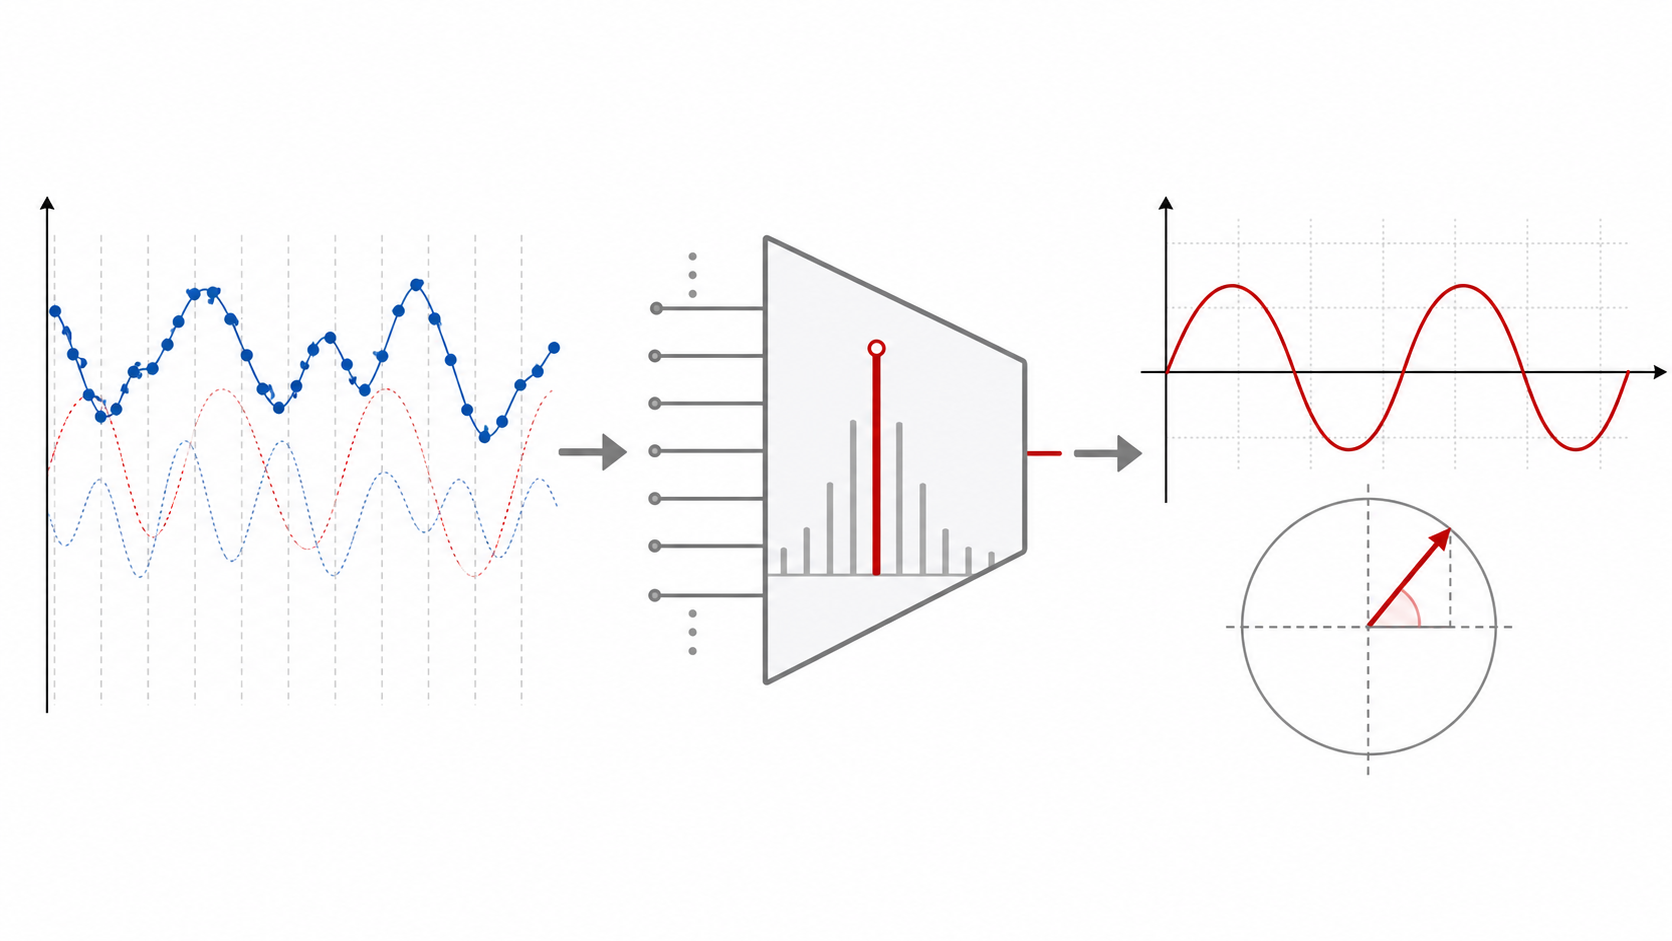
\includegraphics[width=\columnwidth,height=0.62\textheight,keepaspectratio]{obrazky/dft_harmonic_extraction.png}
		\end{column}
	\end{columns}
\end{frame}

\begin{frame}
	\frametitle{Realizace finálního prototypu}
	\small
	\begin{columns}[T]
		\begin{column}{0.28\textwidth}
			\textbf{Finální DPS}
			\begin{itemize}
				\item Šestivrstvá deska
				\item Oddělení analogové a digitální části
				\item Oživení - několik ručních oprav
			\end{itemize}
		\end{column}
		\begin{column}{0.72\textwidth}
			\centering
			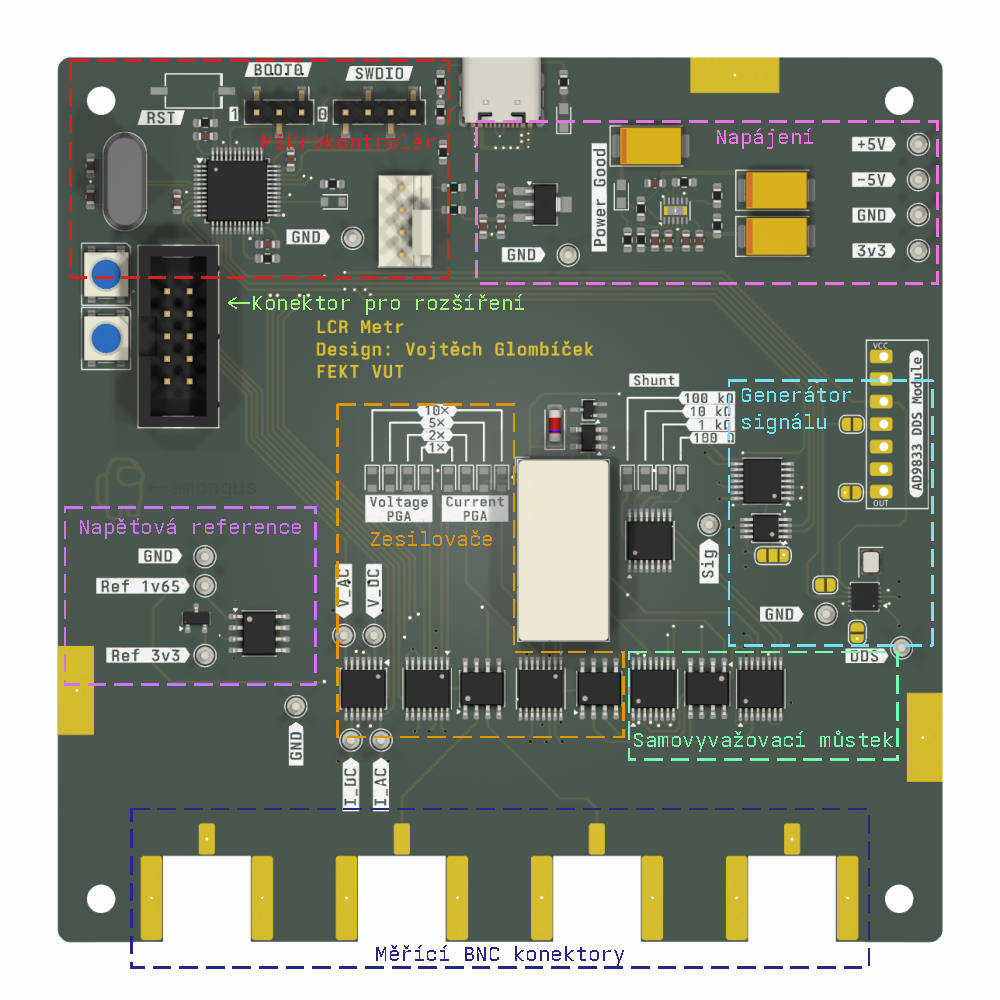
\includegraphics[width=\columnwidth,height=0.76\textheight,keepaspectratio]{obrazky/layout_img.pdf}
		\end{column}
	\end{columns}
\end{frame}

\begin{frame}
	\frametitle{Firmware a PC aplikace}
	\begin{columns}[T]
		\begin{column}{0.43\textwidth}
			\textbf{Firmware}
			\begin{itemize}
				\item Nastavuje analogový frontend
				\item Provádí vzorkování a výpočet impedance
				\item Komunikuje textovými příkazy po sériové lince
			\end{itemize}
			\vspace{0.7em}
				\textbf{PC aplikace}
				\begin{itemize}
					\item Konfigurace měření
					\item Zobrazení naměřených výsledků
					\item Automatizace měření a histogramy
				\end{itemize}
			\end{column}
			\begin{column}{0.57\textwidth}
				\centering
				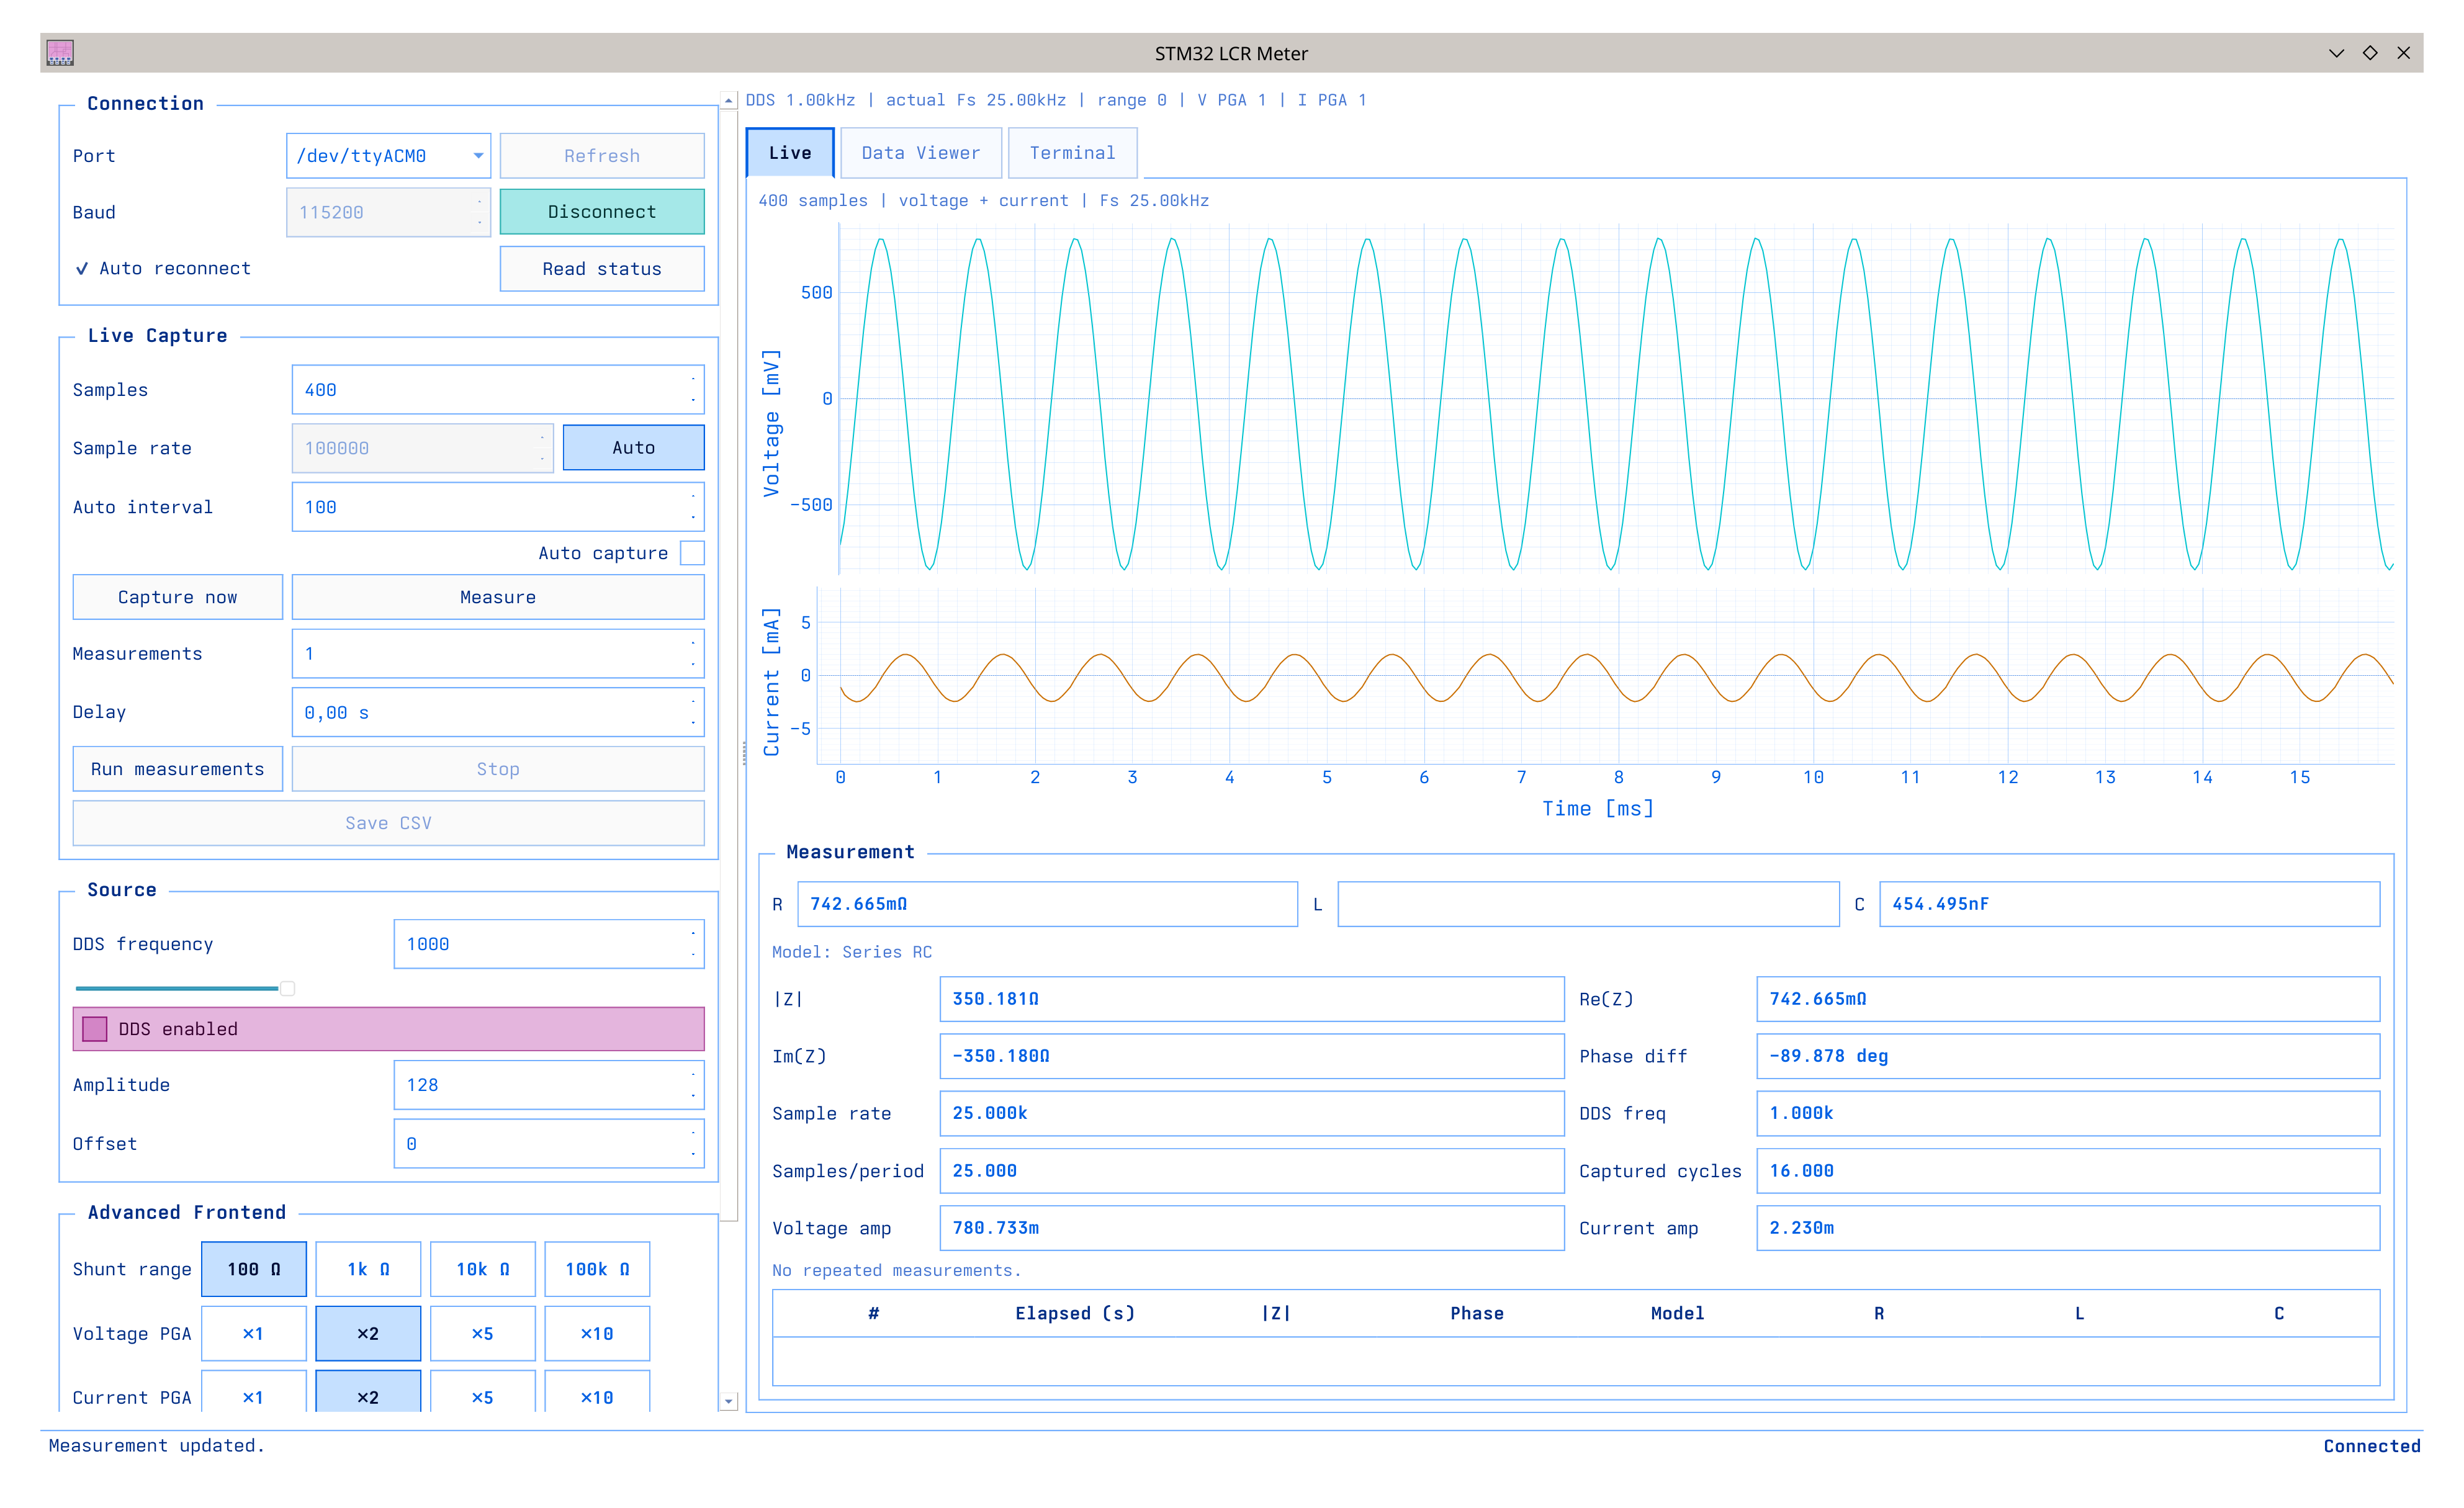
\includegraphics[width=\columnwidth,height=0.62\textheight,keepaspectratio]{obrazky/basic_meas_inv.png}
			\end{column}
	\end{columns}
\end{frame}

\begin{frame}
	\frametitle{Ověření na reálných součástkách}
	\small
	\begin{columns}[T]
			\begin{column}{0.44\textwidth}
				\textbf{Postup měření}
				\begin{itemize}
					\item Sada rezistorů, cívek a kondenzátorů
					\item Měření při 1, 10 a $100\,\mathrm{kHz}$
					\item Srovnání s referenčním LCR metrem BK Precision 880
					\item 1000 vzorků na jedno měření (25 period sinusovky)
				\end{itemize}
			\end{column}
			\begin{column}{0.56\textwidth}
				\centering
				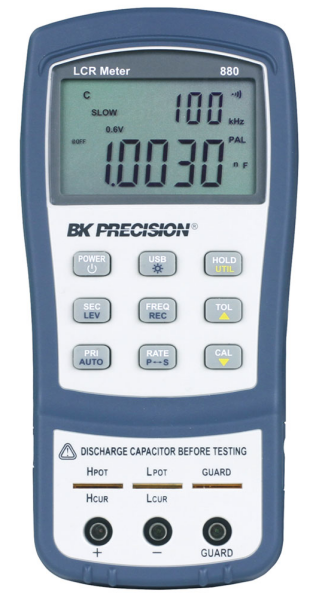
\includegraphics[width=0.46\columnwidth,height=0.34\textheight,keepaspectratio]{obrazky/BK_precision_880.png}
				\vspace{0.25em}

				\begin{tabular}{ccc}
					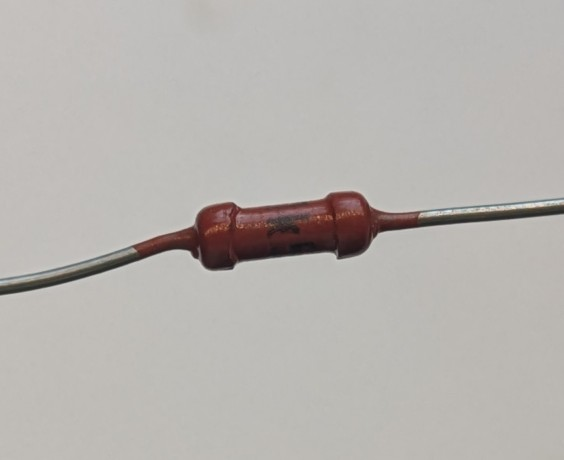
\includegraphics[width=0.25\columnwidth,height=0.12\textheight,keepaspectratio]{obrazky/komponenty/rezistor.jpg} &
					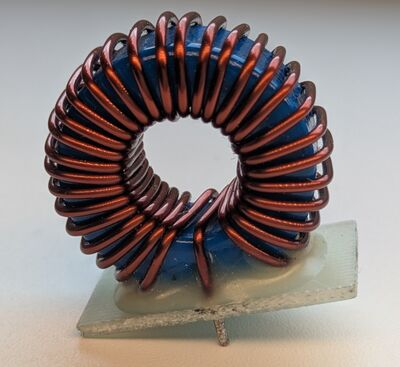
\includegraphics[width=0.25\columnwidth,height=0.12\textheight,keepaspectratio]{obrazky/komponenty/civka_velka.jpg} &
					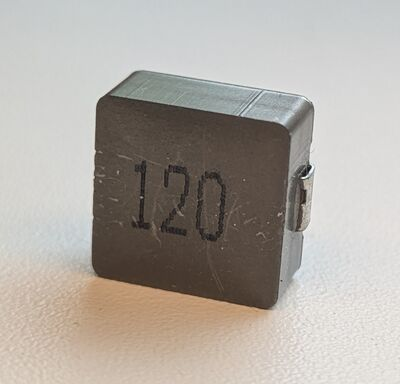
\includegraphics[width=0.25\columnwidth,height=0.12\textheight,keepaspectratio]{obrazky/komponenty/civka_smd.jpg} \\
					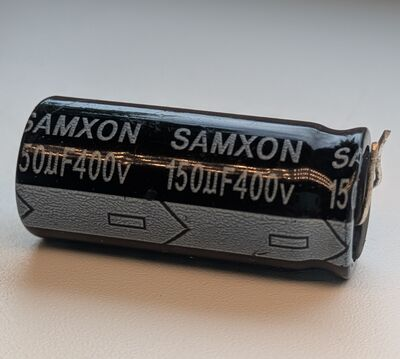
\includegraphics[width=0.25\columnwidth,height=0.12\textheight,keepaspectratio]{obrazky/komponenty/cap_electrolyt.jpg} &
					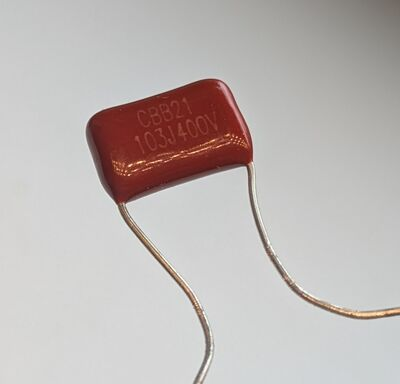
\includegraphics[width=0.25\columnwidth,height=0.12\textheight,keepaspectratio]{obrazky/komponenty/cap_pp_maly.jpg} &
					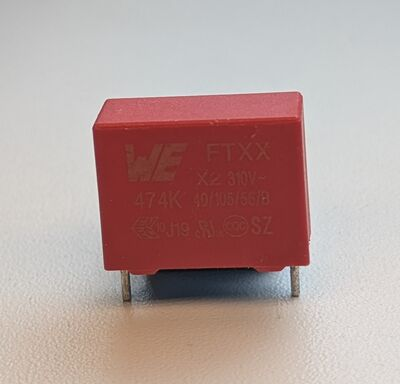
\includegraphics[width=0.25\columnwidth,height=0.12\textheight,keepaspectratio]{obrazky/komponenty/cap_pp_velky.jpg}
				\end{tabular}
			\end{column}
	\end{columns}
\end{frame}

\begin{frame}
	\frametitle{Dosažené výsledky}
	\begin{table}
		\centering
		\Large
		\begin{tabular}{@{}lccc@{}}
			\toprule
			Součástka & 1\,kHz & 10\,kHz & 100\,kHz \\
			\midrule
			Toroidní cívka & $2{,}3\,\%$ & $3{,}7\,\%$ & $2{,}0\,\%$ \\
			SMD cívka $12\,\mu\mathrm{H}$ & $3{,}3\,\%$ & $1{,}3\,\%$ & $0{,}2\,\%$ \\
			Kondenzátor 10\,nF & $0{,}7\,\%$ & $1{,}2\,\%$ & $5{,}7\,\%$ \\
			Kondenzátor 470\,nF & $0{,}5\,\%$ & $1{,}2\,\%$ & $18{,}0\,\%$ \\
			\bottomrule
		\end{tabular}
	\end{table}
\end{frame}

\begin{frame}
	\frametitle{Stabilita a limit 100 kHz}
	\small
	\begin{columns}[T]
		\begin{column}{0.45\textwidth}
			\begin{itemize}
				\item Při 1 a $10\,\mathrm{kHz}$ mají opakovaná měření očekávané rozdělení
				\item Při $100\,\mathrm{kHz}$ se projeví nízký počet vzorků na periodu
			\end{itemize}
				\vspace{0.3em}
				\begin{block}{Hlavní závěr z měření}
					Přístroj je použitelný, ale pro přesnější měření na $100\,\mathrm{kHz}$ je potřeba rychlejší digitalizace.
				\end{block}
		\end{column}
			\begin{column}{0.55\textwidth}
				\centering
					
\includegraphics[width=0.82\columnwidth,height=0.30\textheight,keepaspectratio]{obrazky/komponent_viz/histogramy/toroid_1khz_L.pdf}\par
					\vspace{0.25em}
					
\includegraphics[width=0.82\columnwidth,height=0.30\textheight,keepaspectratio]{obrazky/komponent_viz/histogramy/toroid_100khz_L.pdf}
			\end{column}
	\end{columns}
\end{frame}

\begin{frame}
	\frametitle{Zhodnocení práce}
	\small
	\begin{columns}[T]
		\begin{column}{0.52\textwidth}
			\textbf{V práci jsem:}
			\begin{itemize}
				\item Nastudoval metody měření impedance
				\item Navrhl architekturu LCR metru
				\item Ověřil první prototyp a změnil koncepci vyhodnocení
				\item Navrhl a oživil finální DPS
				\item Napsal firmware a PC aplikaci
				\item Provedl porovnání s referenčním přístrojem
			\end{itemize}
		\end{column}
		\begin{column}{0.48\textwidth}
			\textbf{Další zlepšení}
			\begin{itemize}
				\item Automatické přepínání rozsahů
				\item Kalibrace
				\item Nižší bočníky pro přesnější ESR
				\item Rychlejší ADC
				\item Ochranné obvody
				\item Fyzické ovládání
			\end{itemize}
		\end{column}
	\end{columns}
\end{frame}

\begin{frame}
	\frametitle{Otázka k obhajobě 1}
	\Large
	\begin{block}{}
		Jakým způsobem byste implementoval kalibrační proceduru pro navržený měřič impedance (např. open/short/load)? Jaký dopad byste očekával na výslednou přesnost v celém měřicím pásmu?
	\end{block}
\end{frame}

\begin{frame}
	\frametitle{Odpověď 1: Kalibrace}
	\large
	\begin{itemize}
		\item \textbf{Open, short} -- Kalibrace parazitní impedance přístroje
		\item \textbf{Load} -- Kalibrace chyby etalonem
		\item Kalibrace pro každý rozsah
		\item Uložení korekčních konstant v paměti
		\item Očekávaná přesnost 1-2\%
	\end{itemize}
\end{frame}

\begin{frame}
	\frametitle{Otázka k obhajobě 2}
	\Large
	\begin{block}{}
		Který zdroj chyby považujete ve vašem řešení za dominantní v různých částech měřicího rozsahu (např. nízké vs. vysoké impedance) a jak by bylo možné jeho vliv minimalizovat?
	\end{block}
\end{frame}

\begin{frame}
	\frametitle{Odpověď 2: Dominantní chyby}
	\large
	\begin{itemize}
		\item \textbf{Velikost hodnoty bočníku} -- Měl by být řádově stejný jako měřená impedance
		\item \textbf{Nepřesnost hodnoty bočníku a zisku zesilovače} -- Kalibrace etalonem
		\item \textbf{Omezený měřicí proud} -- Nízké impedance působí jako zkrat; řešení výkonnějším OpAmpem nebo výkonovým stupněm
		\item \textbf{Omezená vzorkovací frekvence} -- Při 100 kHz málo vzorků na periodu, omezené rozlišení měření fáze; řešení - rychlejší ADC
	\end{itemize}
\end{frame}

\begin{frame}[c]
	\frametitle{\mbox{ }}
	\begin{center}
		{\Huge Děkuji za pozornost}
	\end{center}
\end{frame}

\end{document}
